\part{Week 4}
\chapter{Distance measures for quantum information}
We'll try to quantify how two information items are similar, how information is preserved over a process etc. For this, we'll define two classes \textit{distance measures}, \textit{static distance} which is how close two quantum states are, and \textit{dynamic distance} which is how well information is stored over a process. We'll define static distance properly first then build up dynamic distnance with it. Two widely used distance measures currently are \textit{trace distance} and \textit{fidelity}.

\section{Distance measures for classical information}
\textit{Hamming distance} is defined to quantify distance between two bit strings. It's equal to number of mismatching bits (eg. $\text{Hamming}(1011,0010)=2$. But this relies on labelling which we don't have in our Hilbert space arena of quantum mechanics.

We can define a classical information source as a random variable over the set of possible outcomes. So we know the probabilities of getting a given output. In this notion, we can compare two information sources with same index set using a distance measure known as \textit{trace distance}, defined as
\begin{equation}
    D(p_x, q_x) = \frac{1}{2}\sum_x |p_x-q_x|
\end{equation}
where $\{ p_x \}$ and $\{ q_x \}$ are probability distributions of both sources. This is also known as the \textit{$L_1$ distance} or \textit{Kolmogorov distance}. Trace because we use trace when we define this for quantum systems. This is a metric since it satisfies symmetricity ($D(x,y)=D(y,x)$) and triangle inequality ($D(x,y)\leq D(x,z)+D(y,z)$.

\textit{Fidelity}, a second measure is described by
\begin{equation}
    F(p_x, q_x) = \sum \sqrt{p_xq_x}
\end{equation}
This is not a metric as shown by it's physical interpretation in figure \ref{fig:fidelity-distance}.
\begin{figure}
    \centering
    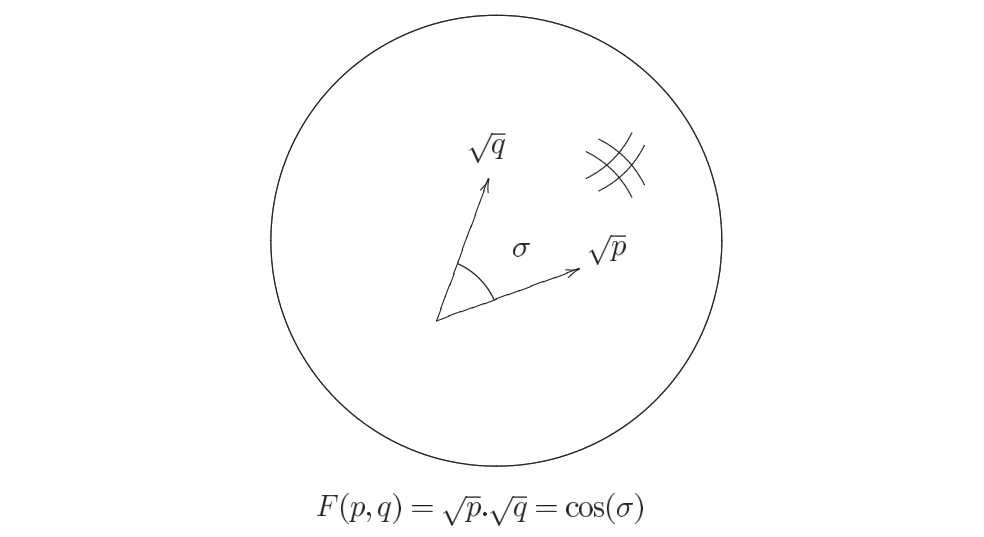
\includegraphics[width=0.9\textwidth]{images/fidelity_distance.png}
    \caption{$F(p_x,q_x)$ can be seen as dot product between $\sqrt{p}$ and $\sqrt{q}$, each of them lie on a unit sphere since $\sum_x \left( \sqrt{p_x} \right)^2 = 1$ and $\sum_x \left( \sqrt{q_x} \right)^2 = 1$}
    \label{fig:fidelity-distance}
\end{figure}

A physically motivated operational meaning for trace distance which can be proved is,
\begin{equation}
    D(p_x, q_x) = \max_S |p(S) - q(S)| = \max_S \left| \sum_{x\in S} p_x - \sum_{x \in S} q_x \right|
\end{equation}
which is maximum over all subsets over index set. This makes sense because $S$ represents an event which produces maximum difference in outputs. It can also be shown that the absolute value is redundant, i.e
\begin{equation}
    D(p_x, q_x) = \max_S \left( \sum_{x\in S} p_x - \sum_{x \in S} q_x\right)
\end{equation}
Trace distance and fidelity are static distance measures.

For \textit{dynamic measure} of distance, suppose a random variable $X$ is passed through a noise channel to produce $Y$ shown by Markov process $X\longrightarrow Y$, a dynamic measure showing how much information is preserved is $p(X\neq Y)$. This can be done using trace distance, for which let's construct a copy $\Tilde{X}$ of $X$ which is also a random variable. Now $X$ is passed through the channel, leaving output $Y$. The closeness between initial perfectly correlated pair $(\Tilde{X}, X)$ and the pair $(\Tilde{X}, Y)$ can be shown to be
\begin{equation}
    D((\Tilde{X},X), (X, Y)) = p(X\neq Y)
    \label{eq:trace_distance_using_copy}
\end{equation}
This thing we did to calculate $p(X\neq Y)$ is unique to classical mechanics. We can't \textit{directly} calculate quantum analogue of $p(X\neq Y)$ if $X$ and $Y$ exist at different times. We use quantum entanglement to define dynamic measure similar to the construction shown above. 
\begin{figure}[H]
    \centering
    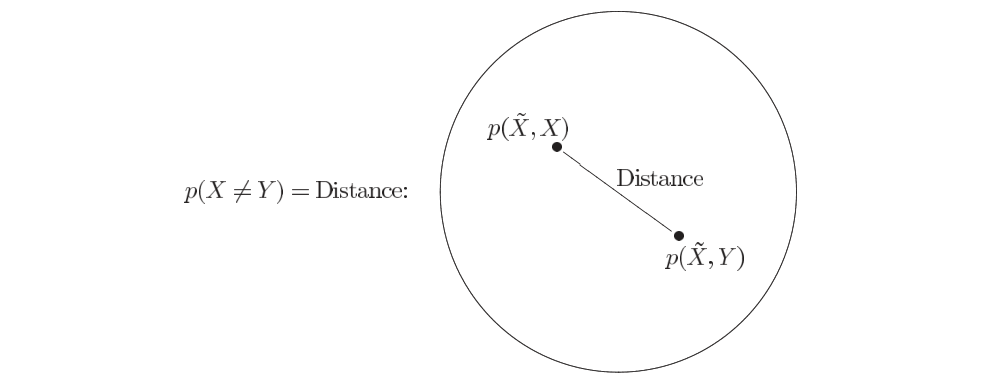
\includegraphics[width=0.8\textwidth]{images/dynamic_measure.png}
    \caption{The probability of an error in the channel is equal to the trace distance between the probability distributions for $( \Tilde{X}, X)$ and $( \Tilde{X}, Y )$.}
    \label{fig:dynamic_measure}
\end{figure}

\section{How close are two quantum states}
We'll see quantum generalizations of trace distance and fidelity.
\subsection{Trace distance}
\textit{Trace distance} between two quantum states $\rho$ and $\sigma$ is defined as
\begin{equation}
    D(\rho, \sigma) = \frac{1}{2}\text{tr} |\rho-\sigma|
\end{equation}
here $|A|=\sqrt{A^\dag A}$. If $\rho$ and $\sigma$ commute (matrix multiplication), this reduces to classical trace distance. Suppose $\rho$ and $\sigma$ commute, then
\begin{align}
    \rho = \sum_i r_i \op{i};
    \ \ \ 
    \sigma = \sum_i s_i \op{i}
\end{align}
for orthogonal basis $\ket{i}$. Then trace distance becomes
\begin{align}
    D(\rho, \sigma) &= \frac{1}{2}\text{tr}|\rho-\sigma| \\
    &= \frac{1}{2}\text{tr}|(r_i-s_i)\op{i}| \\
    &= D(r_i, s_i)
\end{align}
For qubits in Bloch sphere representation, it becomes nicer. Let
\begin{align}
    \rho = \frac{1+\Vec{r}\Vec{\sigma}}{2};
    \ \ \ 
    \sigma = \frac{1+\Vec{s}\Vec{\sigma}}{2}
\end{align}
then trace distance between $\rho$ and $\sigma$ is
\begin{align}
    D(\rho, \sigma) = \frac{|\Vec{r}-\Vec{s}|}{2}
\end{align}
using the fact that $(\Vec{r}-\Vec{s})\cdot \Vec{\sigma}$ has eigen values $\pm |\Vec{r}-\Vec{s}|$. It can be shown that

\begin{equation}
    D(\rho, \sigma) = \max_P \tr{P(\rho-\sigma)}
\end{equation}
where maximum is over all positive operators $P$, $P\leq I$.

\begin{theorem}
    Let $\{ E_m \}$ me a POVM, with $p_m \equiv \tr{\rho E_m}$ and $q_m \equiv \tr{\sigma E_m}$ be the probability of getting output labelled by $m$. Then
    \begin{equation}
        D(\rho, \sigma) = \max_{\{ E_m \} } D(p_m, q_m)
    \end{equation}
    where maximization is over all POVMs $\{ E_m \}$.
\end{theorem}
It can be shown that this trace distance is also a metric. Here goes another nice theorem

\begin{theorem}
    Suppose $\mathcal{E}$ is a trace preserving quantum operation. Let $\rho$, $\sigma$ be density operators. Then
    \begin{equation}
        D(\E{\rho}, \E{\sigma}) \leq D(\rho, \sigma)
    \end{equation}
\end{theorem}
Thus there exists no physical processes which increases distance between two states.
\begin{figure}[H]
    \centering
    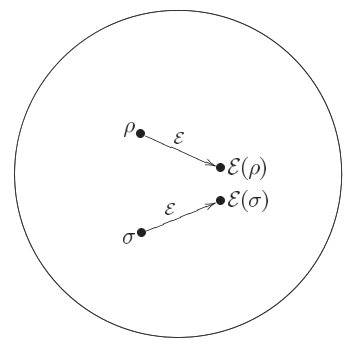
\includegraphics[width=0.4\textwidth]{images/contraction_due_to_operation.png}
    \caption{Trace-preserving quantum operations cause a contraction on the space of density operators.}
    \label{fig:contraction_due_to_operation}
\end{figure}

It can also be showed that
\begin{align}
    D(\rho^A, \sigma^A) \leq D(\rho^{AB}, \sigma^{AB})
\end{align}
intuitively, it's  like things are less differentiable if corresponding parts of them are covered.

\begin{theorem}[\textbf{Strong convexity of trace distance}]
    Let $\{ p_i \}$ and $\{ q_i \}$ be two probability distributions over the same index set, and $\rho_i$, $\sigma_i$ be density operators, also with indices from same index set, then
    \begin{equation}
        D\left( \sum_i p_i\rho_i, \sum_i q_i\sigma_i \right)
        \leq
        D(p_i, q_i) +
        \sum_i p_i D(\rho_i, \sigma_i)
    \end{equation}
    where $D(p_i, q_i)$ is the trace distance between the probability distributions $p_i$ and $q_i$.
\end{theorem}
using this we can show convexity properties of trace distance,
\begin{equation}
    D\left( \sum_i p_i\rho_i , \sigma \right)
    \leq
    \sum_i p_iD(\rho_i, \sigma)
\end{equation}
Also, any trace-preserving quantum operation $\mathcal{E}$ has a fixed point $\rho$ such that $\E{\rho} = \rho$.

\subsection{Fidelity}
\textit{Fidelity} is not a metric on  density operators but does give rise to a useful metric. Fidelity of state $\rho$ and $\sigma$ is defined as
\begin{equation}
    F(\rho, \sigma) \equiv \text{tr}\sqrt{\rho^{1/2}\sigma \rho^{1/2}}
\end{equation}
when $\rho$ and $\sigma$ commute, then
\begin{align}
    \rho = \sum_i p_i\op{i};
    \ \ \ \ 
    \sigma = \sum_i s_i\op{i}
\end{align}
for orthoonormal basis $\ket{i}$, we see that
\begin{align}
    F(\rho, \sigma) &= \text{tr}\sqrt{\sum_i r_is_i\op{i}} \\
    &= \text{tr}\left( \sum_i\sqrt{r_is_i}\op{i} \right) \\
    &= \sum_i \sqrt{r_is_i} \\
    &= F(r_i, s_i)
\end{align}
thus, when $\rho$ and $\sigma$ commute, quantum fidelity reduces to classical fidelity between eigenvalue distributions $r_i$, $s_i$ of $\rho$, $\sigma$ respectively. Also the fidelity between a pure state $\qv$ and an arbitrary state $\rho$ is
\begin{align}
    F(\qv, \rho) &= \text{tr}\sqrt{\bra{\psi}\rho\qv \qv \bra{\psi}} \\
    &= \sqrt{\bra{\psi}\rho\qv}
\end{align}
i.e fidelity is square root of overlap between $\qv$ and $\rho$.

There's no similar Bloch sphere representation for fidelity but it does satisfy similar properties like \textit{invariance under unitary transformation} i.e
\begin{align}
    F(U\rho U^\dag, U\sigma U^\dag) = F(\rho, \sigma)
\end{align}

\begin{theorem}[\textbf{Uhlmann's theorem}]
    Suppose $\rho$, $\sigma$ be states of a system $Q$, Let $R$ be a copy of $Q$. Then
    \begin{equation}
        F(\rho, \sigma) = \max_{\qv, \ket{\varphi}} \left| \braket{\psi | \varphi} \right|
    \end{equation}
    where the maximization is over all purifications $\qv$ of $\rho$ and $\ket{\varphi}$ of $\sigma$.
\end{theorem}

\begin{lemma}
    Let $A$ be any operator, $U$ be unitary. Then
    \begin{equation}
        |\tr{AU}| \leq |\tr{A}|
    \end{equation}
    equality is when $U=V^\dag$ when $A=|A|V$ is polar decomposition of $A$.
\end{lemma}
By Uhlmann's formula it can be shown that fidelity is \textit{symmetric} in its inputs i.e $F(\rho, \sigma) = F(\sigma, \rho)$ and also that it's bound, $0 \leq F(\rho, \sigma) \leq 1$. Also $\rho=\sigma \implies F(\rho, \sigma)=1$ else it's less than 1. Quantum fidelity is related to classical fidelity in the following way:
\begin{equation}
    F(\rho, \sigma) = \min_{E_m} F(p_m, q_m)
\end{equation}
where $E_m$ are POVMs, $p_m = \tr{\rho E_m}$, $q_m = \tr{\sigma E_m}$ are probability distributions corresponding to the POVM $\{ E_m \}$. 

We can define \textit{angle} between states $\rho$ and $\sigma$ by
\begin{equation}
    A(\rho, \sigma) = \arccos{F(\rho, \sigma)}
\end{equation}
This is non-negative, symmetric in inputs and zero when $\rho = \sigma$. It can be shown to satisfy triangle inequality, and thus is a metric.
\begin{figure}[H]
    \centering
    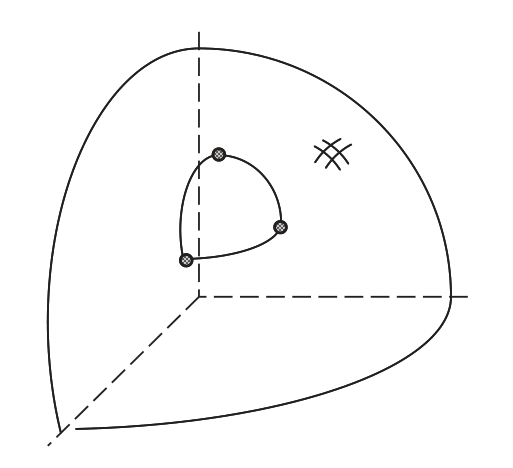
\includegraphics[width=0.5\textwidth]{images/fidelity_angle.png}
    \caption{Angle between unit vectors is a metric}
    \label{fig:fidelity-angle}
\end{figure}
Qualitatively, fidelity behaves like "upside down" of trace distance. It decreases as two states become more distinguishable and vice versa. Fidelity in \textit{non decreasing} as shown by the theorem
\begin{theorem}[\textbf{Monotonicity of fidelity}]
    Suppose $\rho$, $\sigma$ be density operators, and $\mathcal{E}$ is a trace-preserving operation, then
    \begin{equation}
        F(\E{\rho}, \E{\sigma}) \geq F(\rho, \sigma)
    \end{equation}
\end{theorem}
Angles we've defined above follow \textbf{contractivity} which is $A(\E{\rho}, \E{\sigma}) \leq A(\rho, \sigma)$, there's also \textit{strong concavity} of fidelity like trace distance
\begin{theorem}[\textbf{Strong concavity of fidelity}]
    Let $p_i$, $q_i$ be probability distributions over the same index set, $\rho_i$, $\sigma_i$ also indexed by the same index set. Then 
    \begin{equation}
        F \left( \sum_i p_i\rho_i, q_i\sigma_i \right)
        \geq
        \sum_i \sqrt{p_iq_i}F(\rho_i, \sigma_i)
    \end{equation}
\end{theorem}

\subsection{Relationships between distance measures}
Despite their different forms, trace distance and fidelity are closely related. In pure states, they're completely equivalent to each other, to see this consider two pure state $\ket{a}$ and $\ket{b}$, using Gram-schmidt we can find states $\qo$ and $\qi$ such that $\ket{a} = \qo$ and $\ket{b}=\cos{\theta}\qo + \sin{\theta}\qi$. Then $F(\ket{a}, \ket{b}) = |\cos{\theta} |$ and
\begin{align}
    D(\ket{a}, \ket{b}) &= \frac{1}{2}\text{tr} \left|
     \begin{bmatrix}
         1-\cos^2\theta & -\cos{\theta}\sin{\theta} \\
         -\cos{\theta}\sin{\theta} & -\sin^2\theta
     \end{bmatrix} 
    \right|
    \\
    &= |\sin{\theta}| \\
    &= \sqrt{1-F(\ket{a}, \ket{b})^2}    
\end{align}
For mixed states $\rho$, $\sigma$ let $\qv$ and $\ket{\varphi}$ be purifications of $\rho$, $\sigma$ such that $F(\rho, \sigma) = |\braket{\psi | \varphi}| = F(\qv, \ket{\varphi})$. Since trace distance is non-increasing under the partial trace,
\begin{align}
    D(\rho, \sigma) &\leq D(\qv, \ket{\varphi}) \\ 
    &= \sqrt{1-F(\rho, \sigma)^2}
\end{align}
It can be further shown that
\begin{equation}
    1-F(\rho, \sigma) \leq D(\rho, \sigma) \leq \sqrt{1-F(\rho, \sigma)^2}
\end{equation}

\section{How well does a quantum channel preserve information?}
We'll try to quantify how much that state has "changed" from $\qv$ to $\E{\op{\psi}}$ due to an operation $\mathcal{E}$ using the distance measures discussed. Let's look at a simple example how a state changes under depolarizing channel using fidelity
\begin{align}
    F(\qv, \E{\op{\psi}}) &= \sqrt{\bra{\psi}
    \left( p\frac{I}{2} + (1-p)\op{\psi} \right) \qv
    }\\
    &= \sqrt{1-\frac{p}{2}}
\end{align}
it can be clearly seen when we reduce $p$, fidelity get's close to one hence the states becoming more indistinguishable. There's nothing special about fidelity that trace distance doesn't have but we'll stick to this. But in real quantum systems, we don't even know initial state $\qv$ in advance so we try to \textit{minimize} fidelity to get worst-case measure
\begin{equation}
    F_{\min}(\mathcal{E}) \equiv \min_{\qv} F(\qv, \E{\op{\psi}})
\end{equation}
for depolarizing channel it doesn't matter and it's just $\sqrt{1-p/2}$. But for phase damping channel
\begin{equation}
    \E{\rho} = p\rho + (1-p)Z\rho Z
\end{equation}
The fidelity will be
\begin{align}
    F(\qv, \E{\op{\psi}}) &= \sqrt{\bra{\psi} \left( 
    p\op{\psi} + (1-p)Z\op{\psi}Z
    \right)\qv} \\
    &= \sqrt{p + (1-p)\bra{\psi}Z\qv^2}
\end{align}
Now this minimizes when $\frac{\qo+\qi}{\sqrt{2}}$. Thus for phase damping, minimum fidelity becomes
\begin{equation}
    F_{\min}(\mathcal{E}) = \sqrt{p}
\end{equation}
We haven't considered mixed states, but using joint concavity of fidelity it can be shown that allowing mixed states doesn't change $F_{\min}$. Now, we're not only interesting in saving quantum states while transmitting them but we should also look up on when we're computing for example implementing a quantum gate described by $U$. Thus we define \textit{gate-fidelity} as
\begin{equation}
    F(U, \mathcal{E}) = \min_{\qv} F(U\qv, \E{\op{\psi}})
\end{equation}
For example, if we're implementing \textsc{not} gate, but instead implement a noisy operation $\E{\rho} = (1-p)X\rho X + pZ\rho Z$, then gate fidelity is
\begin{align}
    F(X, \mathcal{E}) &=
    \min_{\qv} \sqrt{\bra{\psi}X
    \left( (1-p)X\op{\psi}X + pZ\op{\psi}Z \right)
    X\qv} \\
    &= \min_{\qv} = \sqrt{(1-p) + p\braket{\psi | Y | \psi}^2}
    \\ &= \sqrt{1-p}.
\end{align}

\subsection{Quantum sources of information and the entanglement fidelity}
Even though we've talked a lot about quantum sources we haven't actually defined it. One interesting definition is imagining a stream of quantum systems being produced by some physical process, with their states represented as $\rho_{X_1}, \rho_{X_2}, \dots,$ where $X_j$ are identically distributed random variables and $\rho_j$ is some fixed set of operators. For example, a stream of qubits preparing $\qo$ with $1/2$ probability and $(\qo+\qi)/\sqrt{2}$ with another $1/2$ of probability.

This \textit{ensemble} notion of quantum source leads to notion of \textit{ensemble average fidelity} which captures the idea that source is well preserved under the action of a noisy channel described by trace preserving operator $\mathcal{E}$, as
\begin{equation}
    F = \sum_j p_j F(\rho_j, \E{\rho_j})^2,
\end{equation}
Here, $F=1$ if and only if $\E{\rho_j}=\rho_j$ for all $j$ such that $p_j>0$

The second notion of quantum source is motivated by the fact that a channel preserving information also preserves \textit{entanglement} well. We'll use quantum analogue of what we've considered in \ref{eq:trace_distance_using_copy}.
We'll suppose a quantum system $Q$ entangled with a fictious system $R$, such that the joint state $QR$ is pure. It turns out the result doesn't depend on how this purification is done. Then the system $Q$ is subjected to dynamics described by $\mathcal{E}$.

\begin{figure}[H]
    \centering
    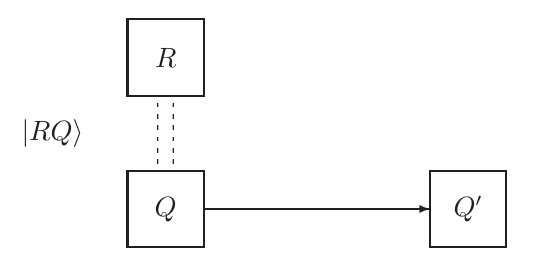
\includegraphics[width=0.5\textwidth]{images/entanglement-fidelity.png}
    \caption{The $RQ$ picture of quantum channel. The initial state of $RQ$ is a pure state.}
    \label{fig:entanglement-fidelity}
\end{figure}

How well is the entanglement preserved by the quantum operation $\mathcal{E}$ is described by \textit{entanglement fidelity} $F(\rho, \mathcal{E})$ which is defined for trace preserving operations $\mathcal{E}$ by
\begin{align}
    F(\rho, \mathcal{E}) &\equiv F(RQ, R'Q')^2 \\
    &= \bra{RQ} \left[ (\mathcal{I}_R \otimes \mathcal{E}) (\op{RQ}) \right] \ket{RQ}
\end{align}
where prime implies after the operation. Entanglement fidelity close to $1$ implies well preserved state and vice versa. One of the important properties of entanglement fidelity is that there's a nice formula to calculate it exactly. Suppose $E_i$ is a set of operation elements for $\mathcal{E}$. Then
\begin{align}
    F(\rho, \mathcal{E})  = \bra{RQ} \rho^{R'Q'} \ket{RQ} = \sum_i |\braket{RQ | E_i | RQ}|^2.
    \label{eq:letsoo}
\end{align}

Suppose $\ket{RQ} = \sum_j \sqrt{p_j}\ket{j}\ket{j}$, where $\rho = \sum_j \op{j}$. Then it can be proved that
\begin{align}
    \bra{RQ} E_i \ket{RQ} = \tr{E_i\rho}
\end{align}
Substituting this is equation \ref{eq:letsoo} we get a useful formula
\begin{equation}
    F(\rho, \mathcal{E}) = \sum_i | \tr{\rho E_i} |^2
\end{equation}

Surprisingly, these two notions are closely related too. This can be seen in two useful properties. First, the entanglement fidelity is a lower bound on the square of the static fidelity between the output and input to the process,
\begin{equation}
    F(\rho, \mathcal{E}) \leq \left[ F(\rho, \E{\rho} \right]^2
\end{equation}
This states that it's harder to preserve entanglement than it is compared to pure states. The second property is that it is a \textit{convex} function of $\rho$. i.e
\begin{equation}
    F\left( \sum_j p_j\rho_j, \mathcal{E} \right) \leq \Bar{F}
\end{equation}
This shows that any channel $\mathcal{E}$ which does a good job of preserving entanglement between a source system $\rho$ and reference system will automatically preserve  the ensemble source described by probabilities $p_j$ and states $\rho_j$ such that $\sum_j p_j\rho_j = \rho$.

I'll try to conclude with most important points yet.
\begin{enumerate}
    \item $0\leq F(\rho, \mathcal{E}) \leq 1$. From properties of static fidelity.
    \item Entanglement fidelity is linear in quantum operation input. This is immediate too.
    \item For pure state inputs, entanglement fidelity is square of static fidelity between input and output,
    \begin{equation}
        F(\qv, \mathcal{E}) = F(\qv, \E{\op{\psi}})^2.
    \end{equation}
    \item $F(\rho, \mathcal{E})=1$ if and only if for all pure state $\qv$ in support of $\rho$
    \begin{equation}
        \E{\op{\psi}} = \op{\psi}.
    \end{equation}
    \item Suppose that $\bra{\psi}\E{\op{\psi}}\qv \leq 1-\eta$ for all $\qv$ in support of $\rho$, for some $\eta$ then $F(\rho, \mathcal{E}) \geq 1-(3\eta/2)$.
\end{enumerate}